Wireless Sensor Networks are being used more and more in almost every field imaginable. Applications generally involve collection and processing of data (either on-site or remote). Applications fields include home automation, agriculture, military, space exploration etc. In order to collect the data, gateway platforms \cite{hill2004platforms,da2011design,da2011design2} are required and most of them are stationary bulky devices or PCs connected to one of the wireless nodes that serve as a base-station. 

We aim to show in this paper that there exists a solution for a truly mobile gateway design that can be used either for collecting data or for debugging large wireless network infrastructures. Our solution involves a system that includes a high-mobility device (such as a quadcopter drone) and a WSN island comprised of nodes that collect data, but are able to store a limited amount of data until the data can be forwarded to the mobile gateway.

We have connected to an AR Parrot Drone 2.0 a SparrowDongle device \cite{voinescu2013lightweight}, a USB stick featuring two micro controllers that can connect to 2.4GHz Zigbee nodes or to our own node design Sparrowv3.2. We will show an overview of the system architecture in Chapter \ref{chap:arch}, the hardware and software implementation in Chapter \ref{chap:impl} and results of using the gateway in Chapter \ref{chap:results}. 



\begin{figure}[ht] \centering
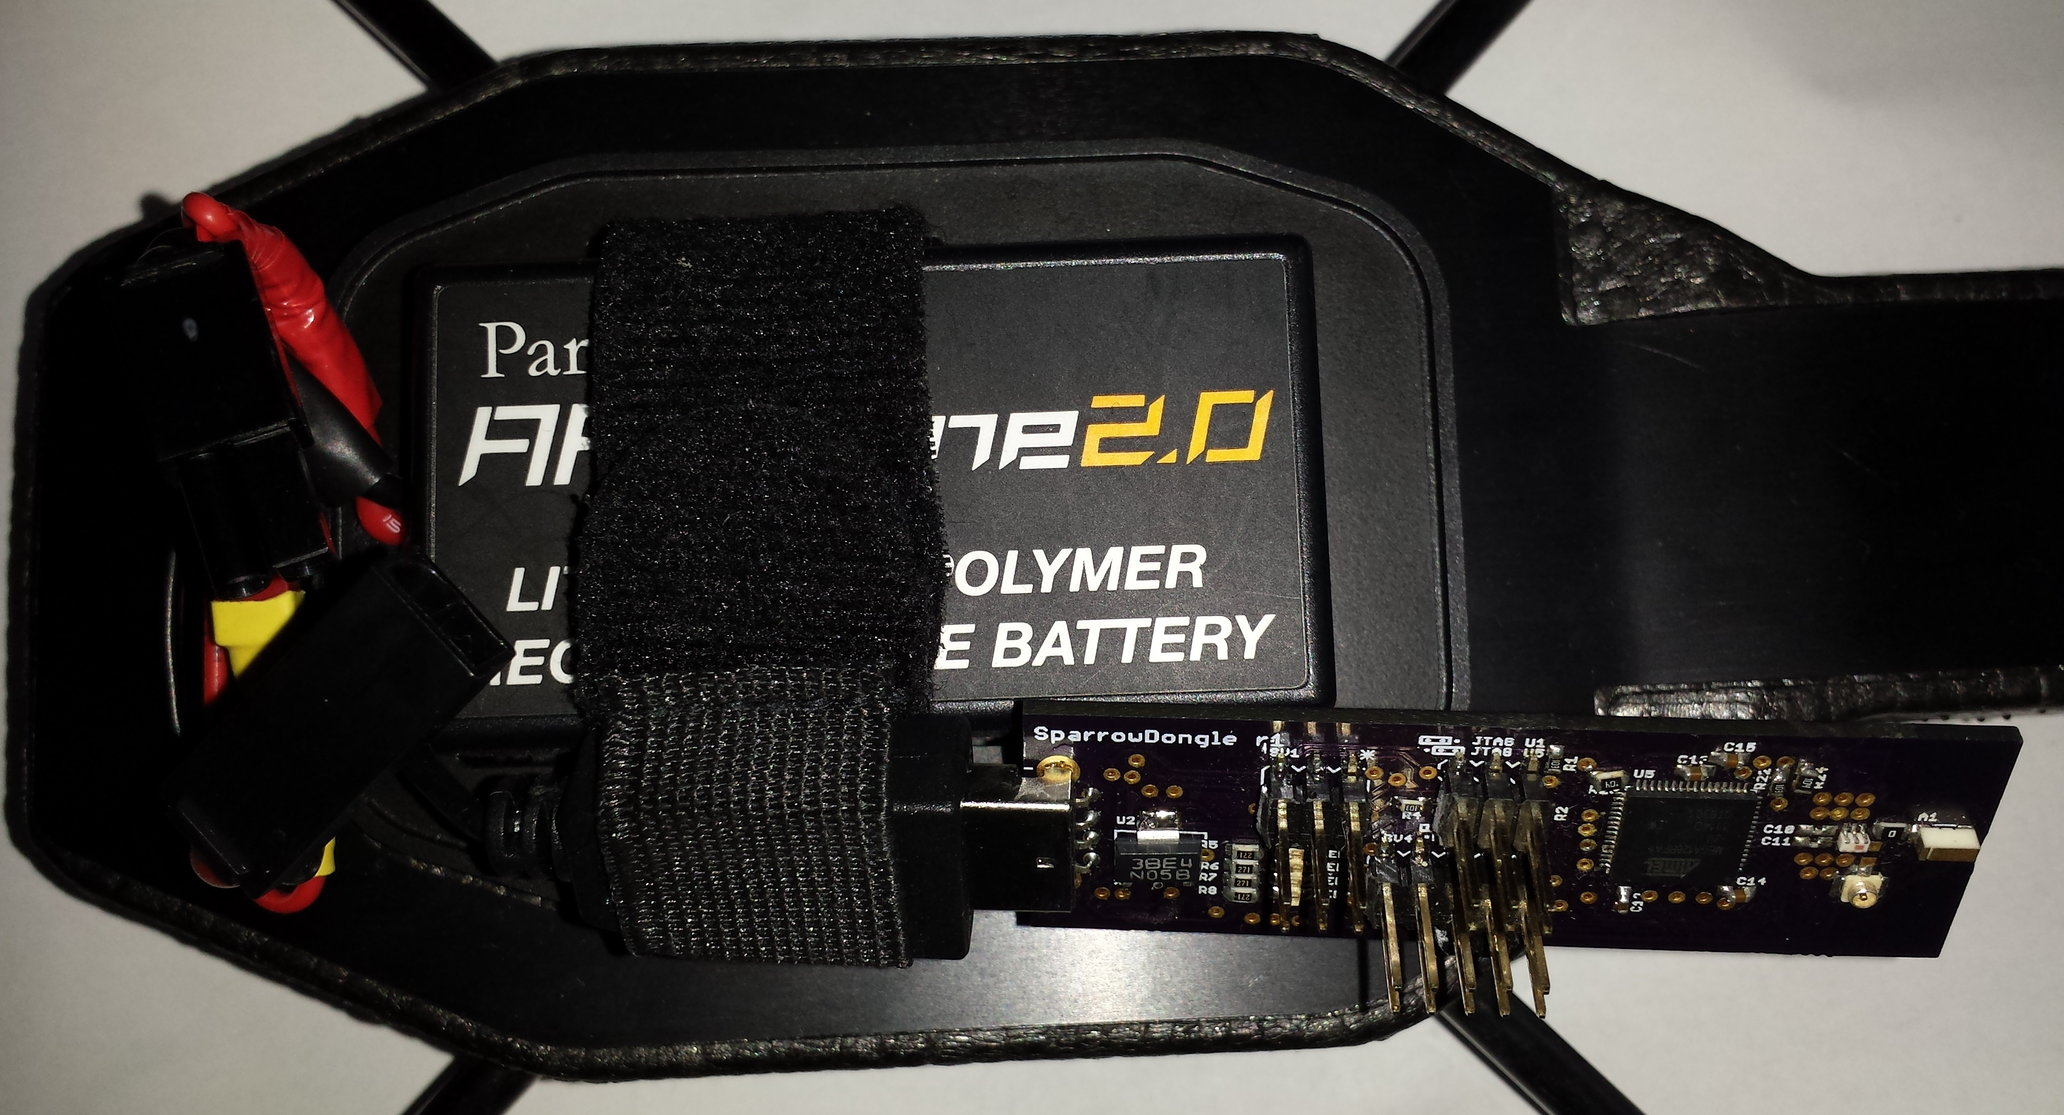
\includegraphics[width=0.45\textwidth]{img/dronedongle.jpg} \caption{SparrowDongle connected to AR Parrot Drone 2.0 } \end{figure}


